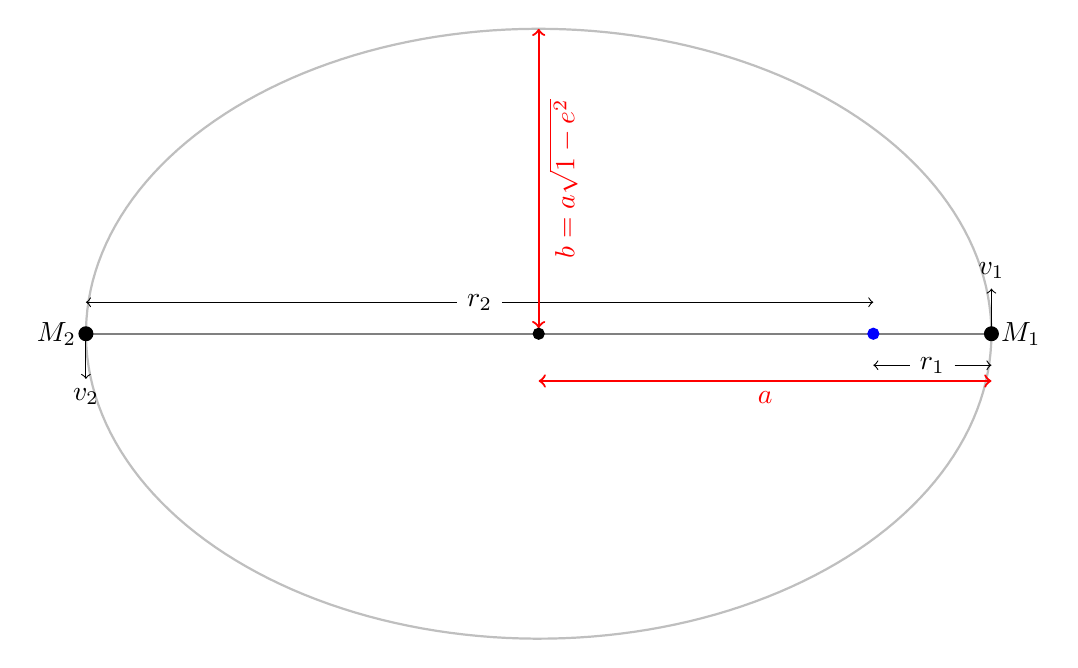
\begin{tikzpicture}
    \def\xOne{-10}    % x-coordinate of first vertex
    \def\yOne{0}    % y-coordinate of first vertex
    \def\xTwo{1.5}    % x-coordinate of second vertex
    \def\yTwo{0}    % y-coordinate of second vertex
    \def\fX{0}      % x-coordinate of focus
    \def\fY{0}      % y-coordinate of focus

    % Calculations
    \pgfmathsetmacro{\Cx}{(\xOne+\xTwo)/2} % Center x
    \pgfmathsetmacro{\Cy}{(\yOne+\yTwo)/2} % Center y
    \pgfmathsetmacro{\xOneMid}{(\xOne+\fX)/2} % midpoint of x1 and barycenter

    \pgfmathsetmacro{\xTwoMid}{(\xTwo+\fX)/2} % midpoint of x2 and barycenter

    \pgfmathsetmacro{\a}{sqrt((\xTwo-\xOne)^2 + (\yTwo-\yOne)^2)/2} % Semi-major axis
    \pgfmathsetmacro{\c}{sqrt((\fX-\Cx)^2 + (\fY-\Cy)^2)} % Distance to focus
    \pgfmathsetmacro{\b}{sqrt(\a^2 - \c^2)} % Semi-minor axis
    \pgfmathsetmacro{\theta}{atan2(\yTwo-\yOne, \xTwo-\xOne)} % Rotation angle

    \pgfmathsetmacro{\xOneArrowOrd}{\xOne+0.1};
    \pgfmathsetmacro{\xTwoArrowOrd}{\xTwo-0.1};

    \pgfmathsetmacro{\xOneArrowX}{\xOneArrowOrd};
    \pgfmathsetmacro{\xTwoArrowX}{\xTwoArrowOrd};

    \pgfmathsetmacro{\xOneArrowY}{\Cy + \a*sin(\theta)*cos(deg(\xOneArrowX)) + \b*cos(\theta)*sin(deg(\xOneArrowX))};

    \pgfmathsetmacro{\xTwoArrowY}{\Cy + \a*sin(\theta)*cos(deg(\xTwoArrowX)) + \b*cos(\theta)*sin(deg(\xTwoArrowX))};

    % Plot the ellipse
    \draw[thick, lightgray, domain=0:360, samples=200]
        plot ({\Cx + \a*cos(\theta)*cos(\x) - \b*sin(\theta)*sin(\x)},
              {\Cy + \a*sin(\theta)*cos(\x) + \b*cos(\theta)*sin(\x)});

    \draw[gray, thick] (\xOne, \yOne) -- (0, 0);
    \draw[gray, thick] (\xTwo, \yTwo) -- (0, 0);
    \filldraw[blue] (0, 0) circle (2pt);

    \node (a) at (\xOneMid, \yOne+0.4) {$r_2$};
    \draw[<-] (\xOne, \yOne+0.4) -- (a);
    \draw[->] (a) -- (\fX, \yOne+0.4);

    \node (b) at (\xTwoMid, \yTwo-0.4) {$r_1$};
    \draw[<-] (\fX, \yTwo-0.4) -- (b);
    \draw[->] (b) -- (\xTwo, \yTwo-0.4);

    \filldraw[black] (\xOne, \yOne) circle (2.5pt) node[anchor=east] {$M_2$};
    \filldraw[black] (\xTwo, \yTwo) circle (2.5pt) node[anchor=west] {$M_1$};

    \node (drawtoB) at (\xTwo, 0.8) {$v_1$};
    \node (drawtoA) at (\xOne, -0.8) {$v_2$};

    \draw[->] (\xOne, \yOne) -- (drawtoA);
    \draw[->] (\xTwo, \yTwo) -- (drawtoB);

    \draw[<->,red, thick] (\Cx, \Cy-0.6) -- (\Cx+\a, \Cy-0.6) node[below, midway] {$a$};
    \draw[<->, red, thick] (\Cx, \Cy+2pt) -- (\Cx, \Cy+\b) node[below, midway, sloped] {$b=a\sqrt{1-e^2}$};
    \filldraw[black] (\Cx, \Cy) circle (2pt);
\end{tikzpicture}